\documentclass[english,notitlepage]{revtex4-1}  % defines the basic parameters of the document
%For preview: skriv i terminal: latexmk -pdf -pvc filnavn



% if you want a single-column, remove reprint

% allows special characters (including æøå)
\usepackage[utf8]{inputenc}
%\usepackage[english]{babel}

%% note that you may need to download some of these packages manually, it depends on your setup.
%% I recommend downloading TeXMaker, because it includes a large library of the most common packages.

\usepackage{physics,amssymb}  % mathematical symbols (physics imports amsmath)
\usepackage{amsmath}
%include{amsmath}
\usepackage{graphicx}         % include graphics such as plots
\usepackage{xcolor}           % set colors
\usepackage{hyperref}         % automagic cross-referencing (this is GODLIKE)
\usepackage{listings}         % display code
\usepackage{subfigure}        % imports a lot of cool and useful figure commands
\usepackage{float}
%\usepackage[section]{placeins}
\usepackage{algorithm}
\usepackage[noend]{algpseudocode}
\usepackage{subfigure}
\usepackage{tikz}
\usetikzlibrary{quantikz}
% defines the color of hyperref objects
% Blending two colors:  blue!80!black  =  80% blue and 20% black
\hypersetup{ % this is just my personal choice, feel free to change things
    colorlinks,
    linkcolor={red!50!black},
    citecolor={blue!50!black},
    urlcolor={blue!80!black}}

%% Defines the style of the programming listing
%% This is actually my personal template, go ahead and change stuff if you want



%% USEFUL LINKS:
%%
%%   UiO LaTeX guides:        https://www.mn.uio.no/ifi/tjenester/it/hjelp/latex/
%%   mathematics:             https://en.wikibooks.org/wiki/LaTeX/Mathematics

%%   PHYSICS !                https://mirror.hmc.edu/ctan/macros/latex/contrib/physics/physics.pdf

%%   the basics of Tikz:       https://en.wikibooks.org/wiki/LaTeX/PGF/Tikz
%%   all the colors!:          https://en.wikibooks.org/wiki/LaTeX/Colors
%%   how to draw tables:       https://en.wikibooks.org/wiki/LaTeX/Tables
%%   code listing styles:      https://en.wikibooks.org/wiki/LaTeX/Source_Code_Listings
%%   \includegraphics          https://en.wikibooks.org/wiki/LaTeX/Importing_Graphics
%%   learn more about figures  https://en.wikibooks.org/wiki/LaTeX/Floats,_Figures_and_Captions
%%   automagic bibliography:   https://en.wikibooks.org/wiki/LaTeX/Bibliography_Management  (this one is kinda difficult the first time)
%%   REVTeX Guide:             http://www.physics.csbsju.edu/370/papers/Journal_Style_Manuals/auguide4-1.pdf
%%
%%   (this document is of class "revtex4-1", the REVTeX Guide explains how the class works)


%% CREATING THE .pdf FILE USING LINUX IN THE TERMINAL
%%
%% [terminal]$ pdflatex template.tex
%%
%% Run the command twice, always.
%% If you want to use \footnote, you need to run these commands (IN THIS SPECIFIC ORDER)
%%
%% [terminal]$ pdflatex template.tex
%% [terminal]$ bibtex template
%% [terminal]$ pdflatex template.tex
%% [terminal]$ pdflatex template.tex
%%
%% Don't ask me why, I don't know.

\begin{document}

\title{FYS-STK4155 Week 36}      % self-explanatory
\author{Janita Ovidie Sandtrøen Willumsen}          % self-explanatory
\date{\today}                             % self-explanatory
\noaffiliation                            % ignore this, but keep it.


\maketitle 
    
% \textit{List a link to your github repository here!}
    
\section*{Exercise 1a}
\begin{figure}[H]
    \centering
    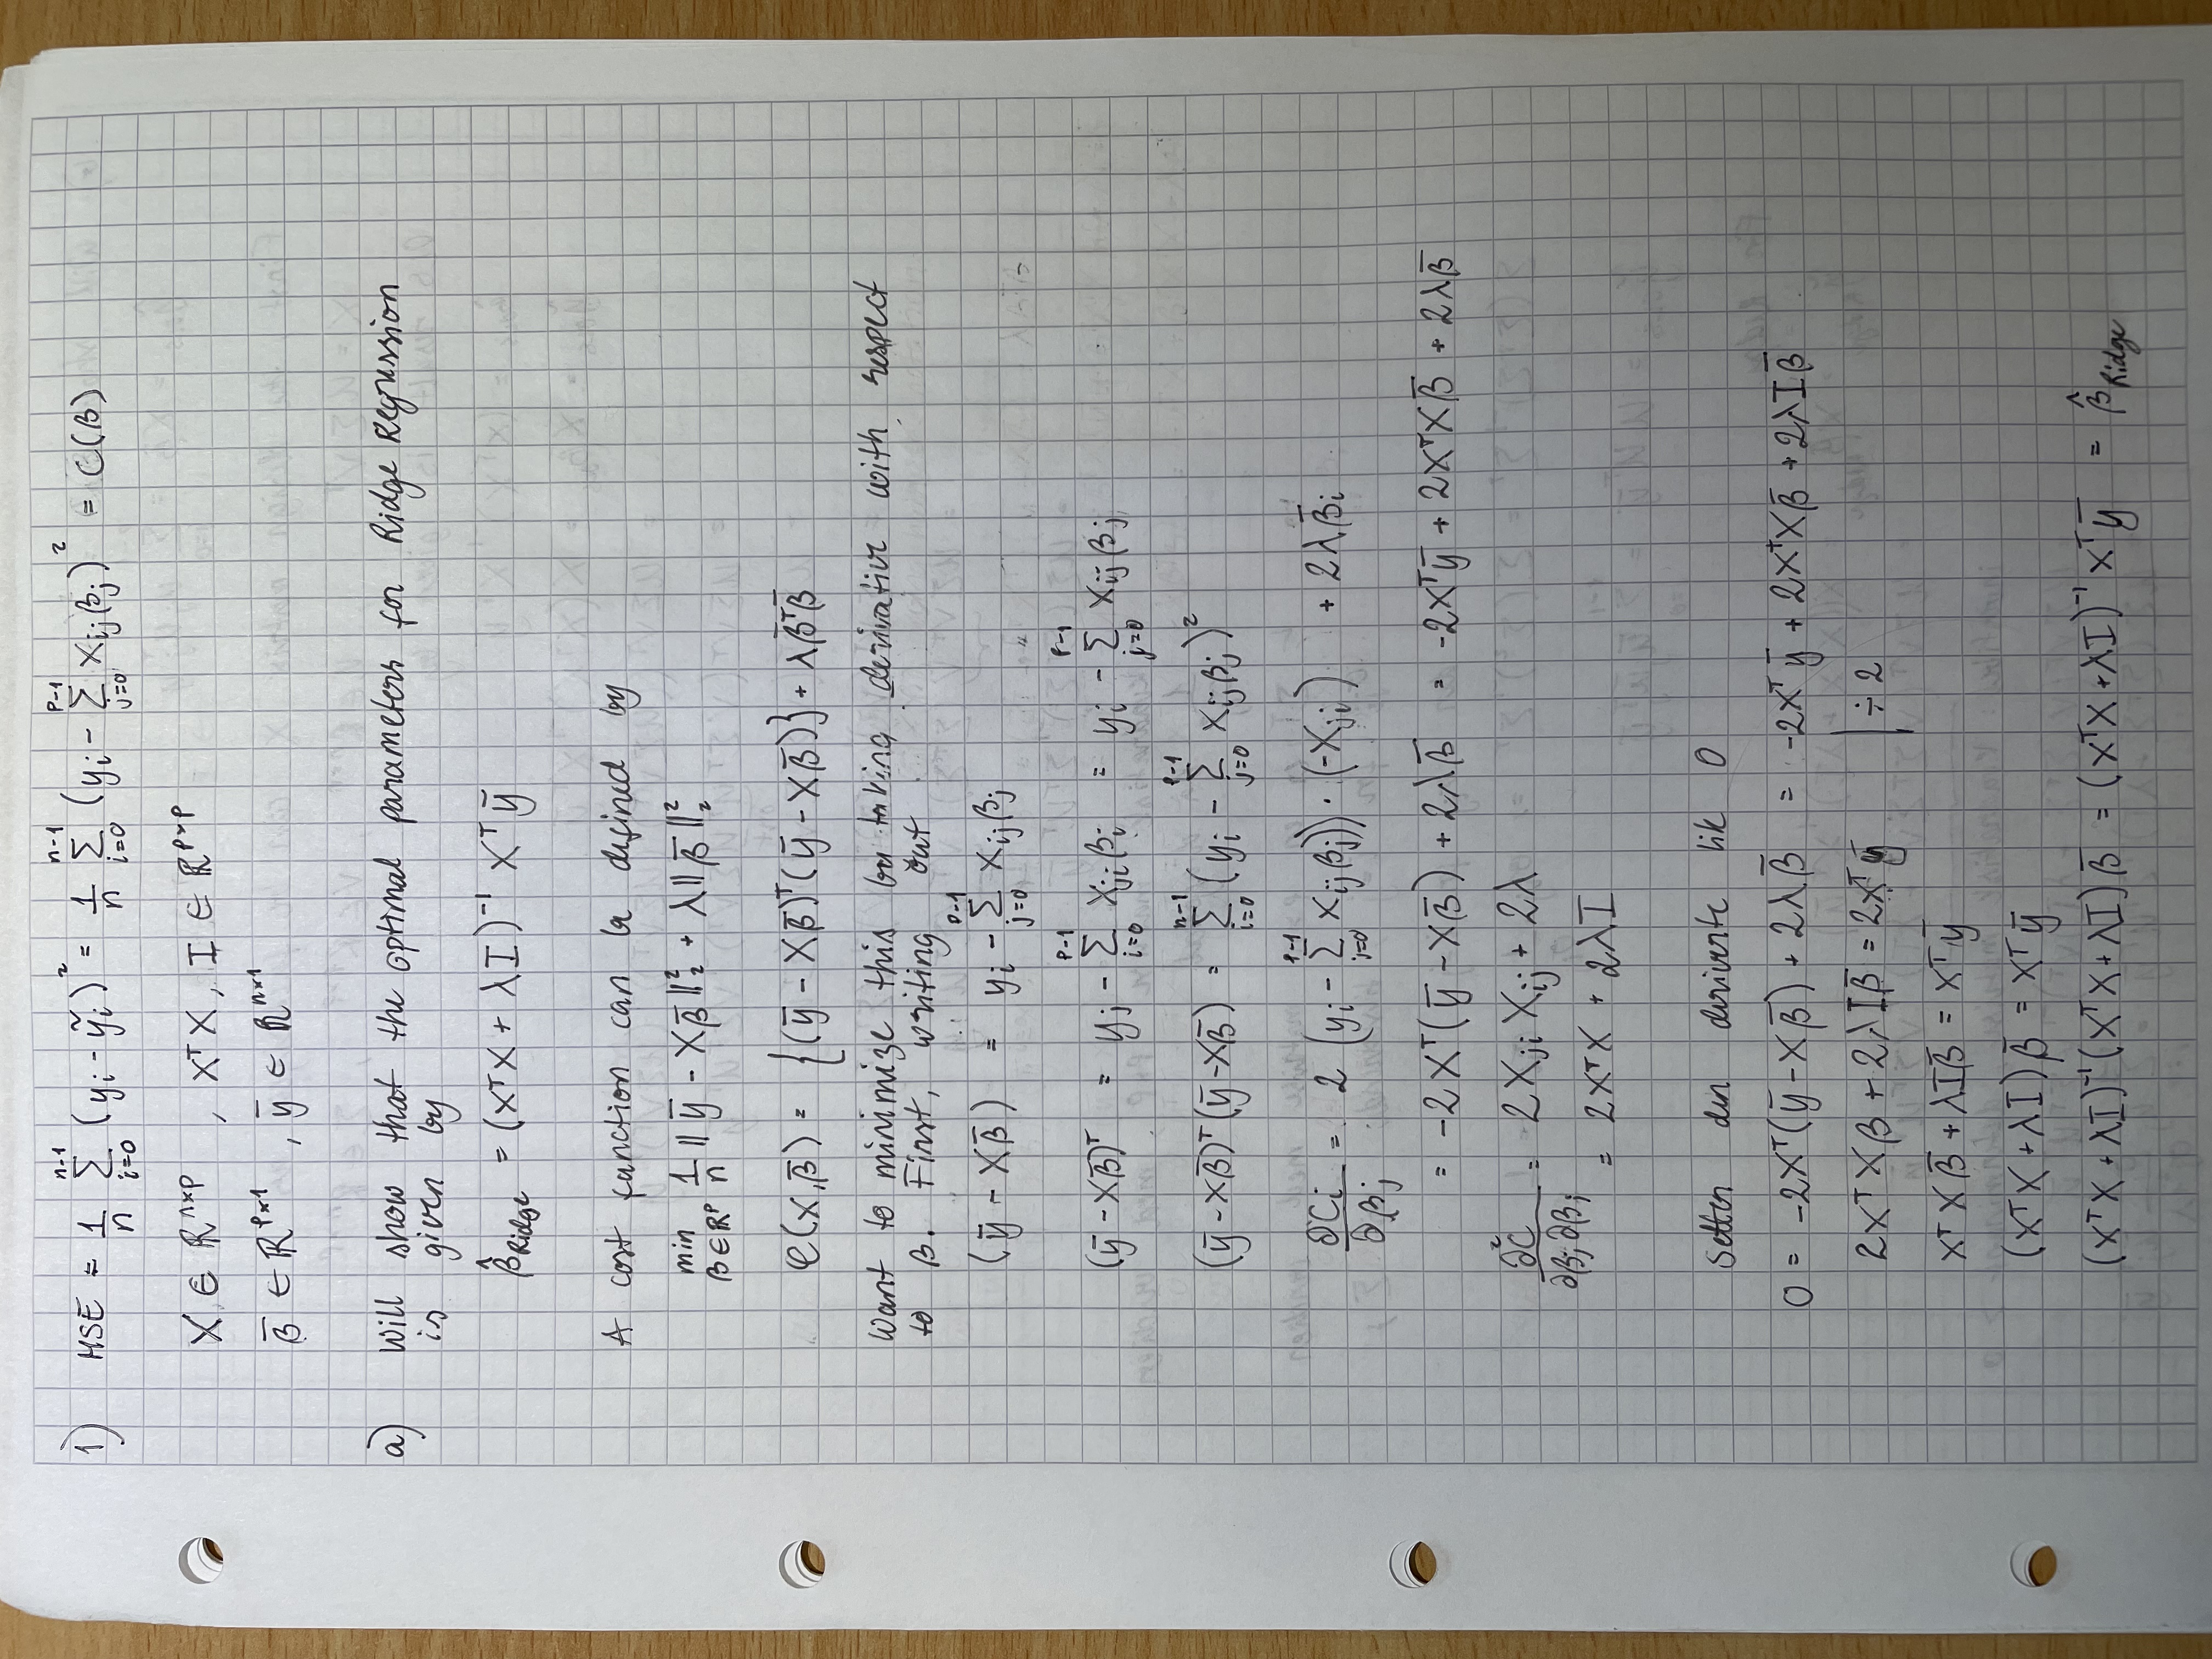
\includegraphics[angle=-90, width=\linewidth]{Week 36/36_1.jpg}
\end{figure}

\section*{Exercise 1b}
\begin{figure}[H]
    \centering
    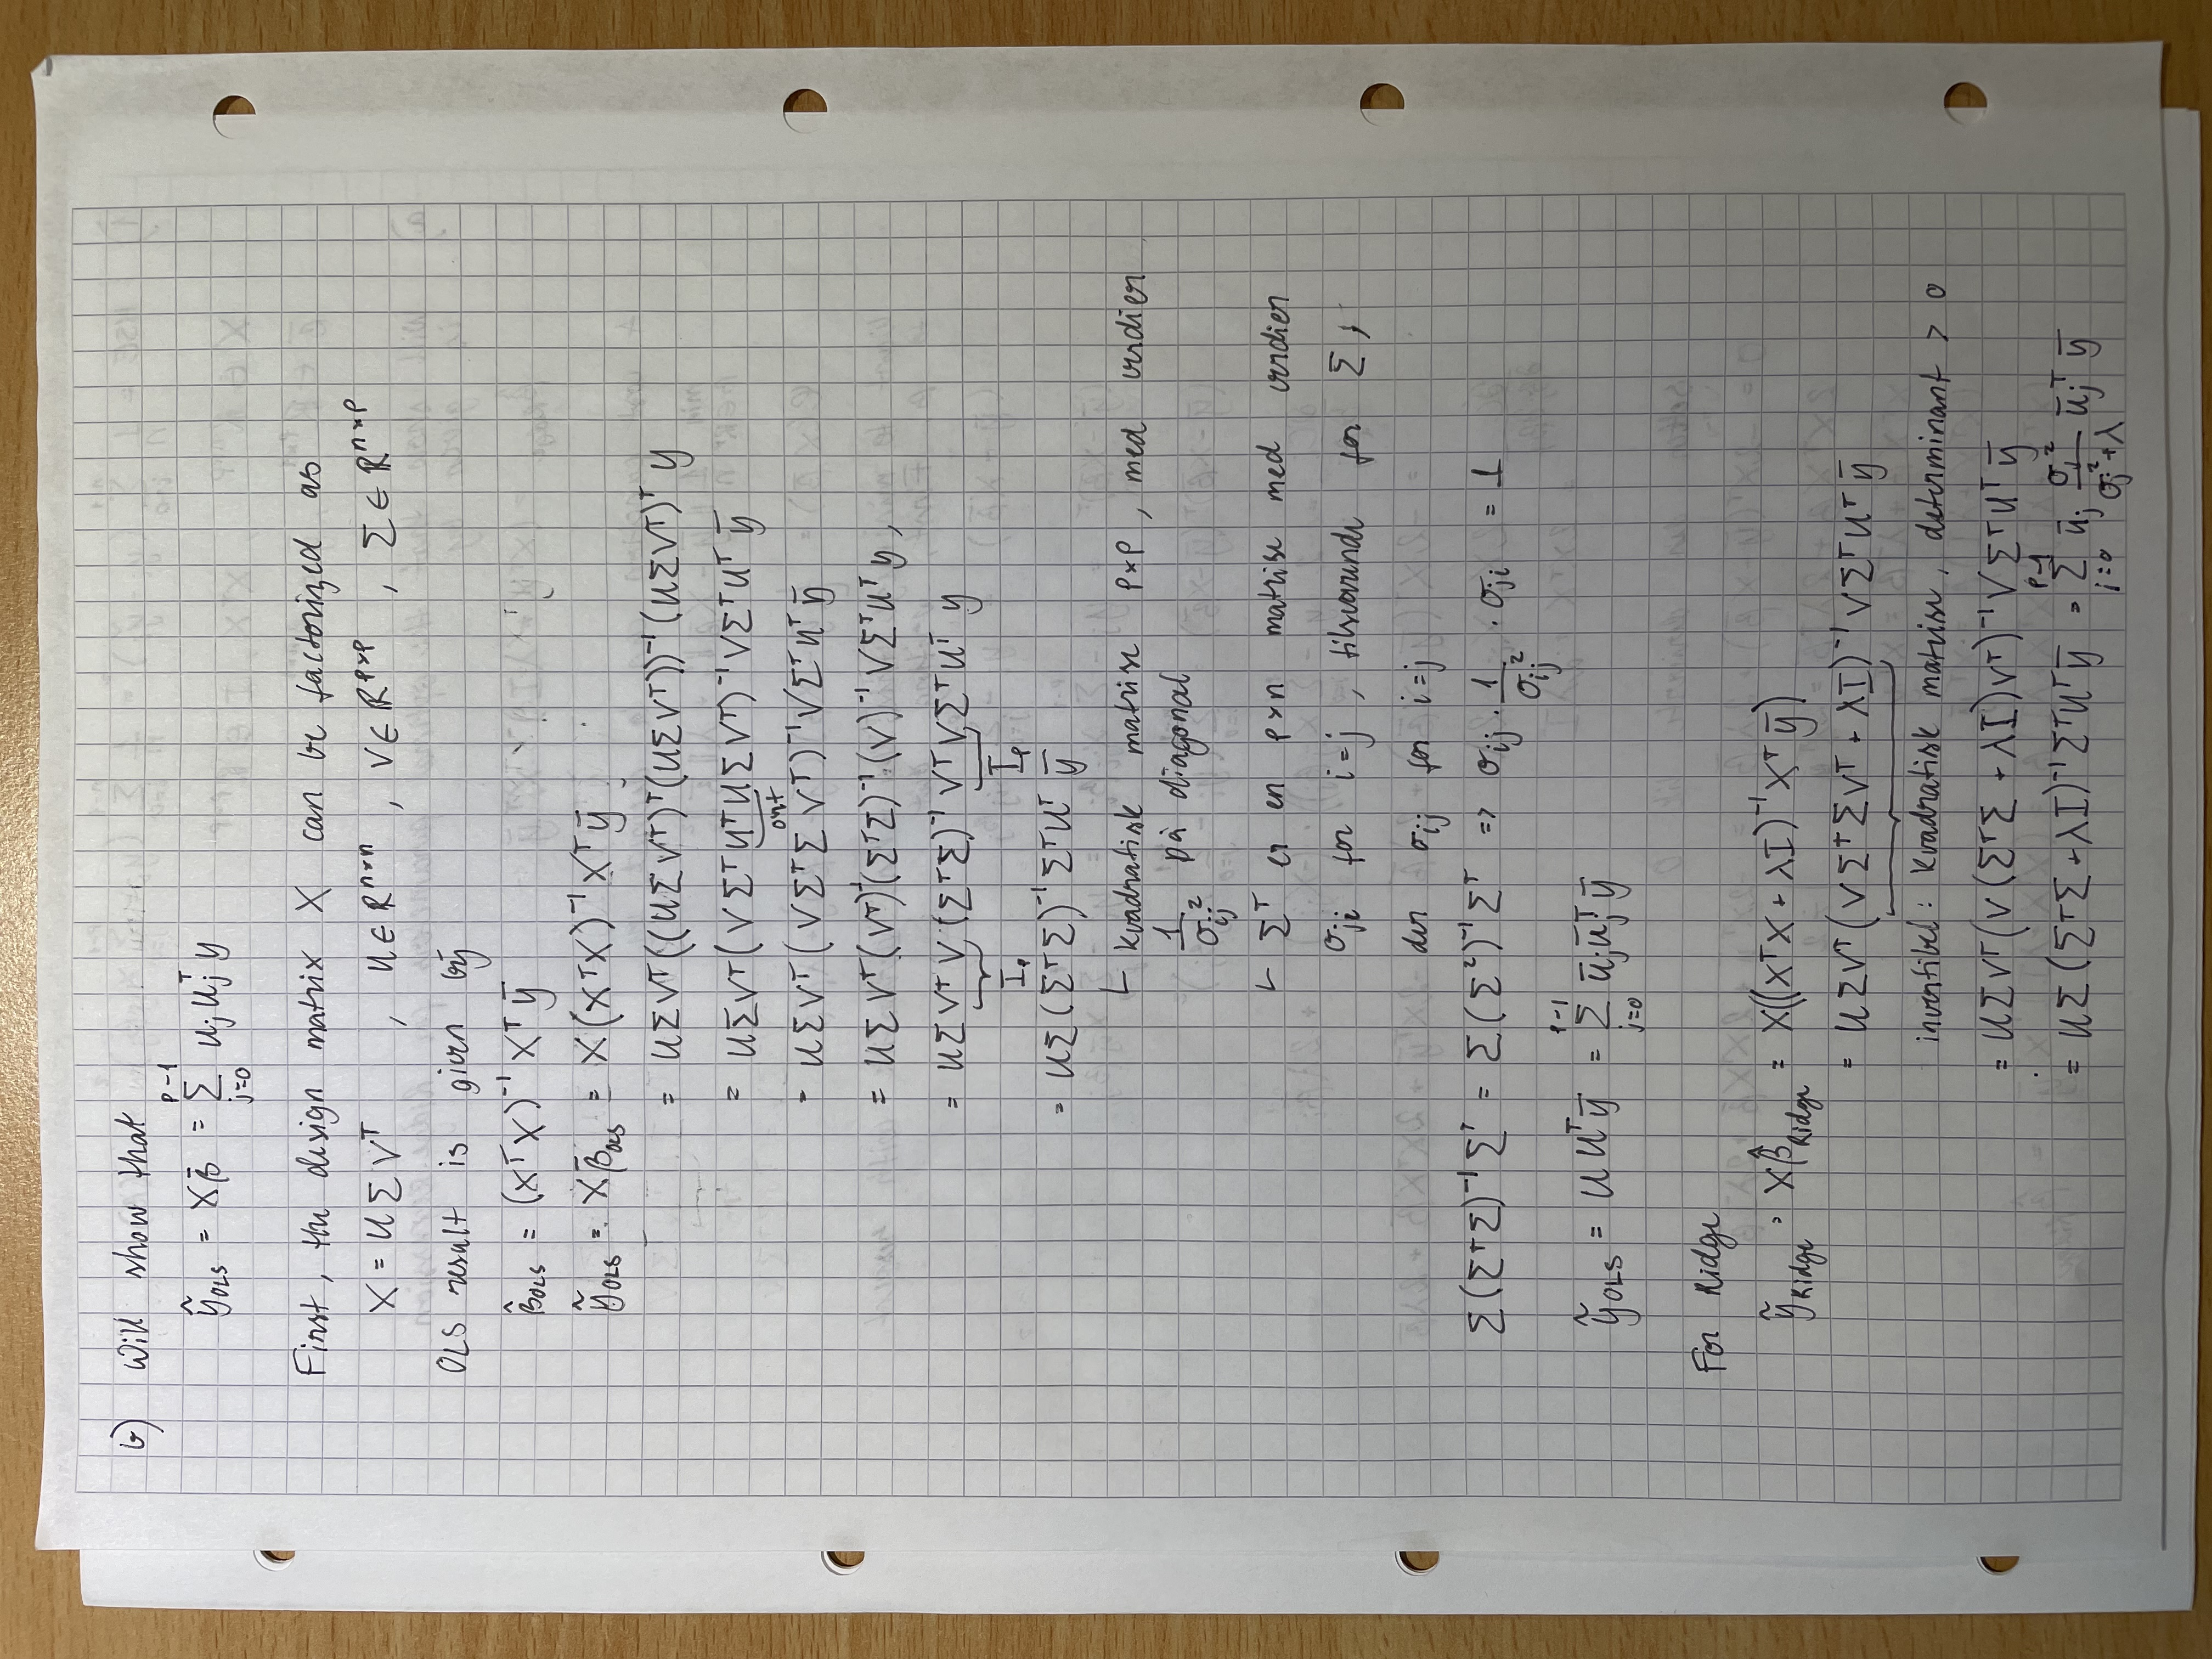
\includegraphics[angle=-90, width=\linewidth]{Week 36/36_2.jpg}
\end{figure}

\section*{Exercise 2}
For smaller values of $\lambda$ the mean squared error of ridge regression is closer to ordinary least squares. This is expected as $\lambda$ close to zero would give the same $\beta$ as for OLS.
In addition, by increasing the polynomial order MSE decrease for both Ridge and OLS.

\lstinputlisting[language=Python]{fys-stk4155-week-36.py}

\begin{table}[H]
    \centering
    \caption{Output from running script with polynomial order 5, 10, and 15.}
    \begin{tabular}{|c|c|c|c|c|}
        \hline
        $\lambda$ &  & $p=5$ & $p=10$ & $p=15$ \\ [0.5ex]
        \hline
        0 & Train & 0.022483 & 0.010269 & 0.009284 \\
        0 & Test & 0.022759 & 0.012183 & 0.013650 \\
        0.0001 & Train & 0.022483 & 0.010269 & 0.009284 \\
        0.0001 & Test & 0.022759 & 0.012184 & 0.013645 \\
        0.001 & Train & 0.022483 & 0.010269 & 0.009284 \\
        0.001 & Test & 0.022757 & 0.012185 & 0.013598 \\
        0.01 & Train & 0.022483 & 0.010270 & 0.009310 \\
        0.01 & Test & 0.022743 & 0.012205 & 0.013270 \\
        0.1 & Train & 0.022487 & 0.010369 & 0.009562 \\
        0.1 & Test & 0.022609 & 0.012450 & 0.012729 \\
        1.0 & Train & 0.022892 & 0.012649 & 0.011192 \\
        1.0 & Test & 0.021629 & 0.014356 & 0.014077 \\
        \hline
    \end{tabular}\label{tab:output_table}
\end{table}


\end{document}